% Freight rate prediction report. Build with `python -m src.report`; every number and
% table comes from generated/ (written by src/report.py from artifacts/), so edit the
% prose here and the numbers there regenerate with the results.
\documentclass[10pt,letterpaper]{article}

\usepackage[T1]{fontenc}
\usepackage[utf8]{inputenc}
\usepackage{XCharter}
\usepackage[scale=0.95]{sourcesanspro}
\usepackage[charter,vvarbb]{newtxmath}
\usepackage{textcomp}
\usepackage[margin=0.9in,top=0.8in,bottom=0.85in]{geometry}
\usepackage{microtype}
\usepackage{graphicx}
\usepackage{array}
\usepackage{booktabs}
\usepackage[table]{xcolor}
\usepackage{caption}
\usepackage{enumitem}
\usepackage{titlesec}
\usepackage{fancyhdr}
\usepackage{float}
\usepackage[hidelinks]{hyperref}

\graphicspath{{figures/}{../scorer_results/}}
\definecolor{ink2}{HTML}{52514E}
\definecolor{accent}{HTML}{1C5CAB}
\definecolor{chosen}{HTML}{EEF3FA}

\titleformat{\section}{\sffamily\bfseries\large\color{accent}}{\thesection}{0.6em}{}
\titlespacing*{\section}{0pt}{1.1em}{0.4em}
\titleformat{\paragraph}[runin]{\bfseries}{}{0pt}{}[.]
\titlespacing*{\paragraph}{0pt}{0.5em}{0.5em}
\captionsetup{font={small,color=ink2},labelfont=bf,skip=4pt}
\setlist[itemize]{leftmargin=1.2em,itemsep=2pt,topsep=3pt}
\setlength{\parskip}{4pt}
\setlength{\parindent}{0pt}
\renewcommand{\arraystretch}{1.12}
\pagestyle{fancy}
\fancyhf{}
\renewcommand{\headrulewidth}{0pt}
\fancyfoot[L]{\small\color{ink2}Freight rate prediction}
\fancyfoot[R]{\small\color{ink2}\thepage}

\newcommand{\MI}{\texttt{market\_index}}
\newcommand{\QS}{\texttt{quote\_signal}}
\newcommand{\PR}{\texttt{posted\_rate}}

% Generated by src/report.py from artifacts/. Do not edit.
\newcommand{\HybAvgMAE}{\$85.2}
\newcommand{\HybHtwoMAE}{\$88.5}
\newcommand{\HybAvgCMAPE}{1.33\%}
\newcommand{\HybHtwoCMAPE}{1.37\%}
\newcommand{\HybAvgMAPE}{3.83\%}
\newcommand{\HybOctBias}{1.0\%}
\newcommand{\BlendAvgMAE}{\$113.7}
\newcommand{\LgbmAvgMAE}{\$113.8}
\newcommand{\LgbmNoQsAvgMAE}{\$102.9}
\newcommand{\HybQsAvgMAE}{\$86.7}
\newcommand{\HybUntunedAvgMAE}{\$87.1}
\newcommand{\HybNoMiHtwoCMAPE}{4.76\%}
\newcommand{\RmseMin}{\$623}
\newcommand{\RmseMax}{\$640}
\newcommand{\SeedsHtwo}{\$88.5 / \$88.5 / \$88.5}
\newcommand{\RndHyb}{\$91.5}
\newcommand{\RndLgbm}{\$95.3}
\newcommand{\FwdHyb}{\$95.4}
\newcommand{\FwdLgbm}{\$110.6}
\newcommand{\UcHyb}{\$88.2}
\newcommand{\UcLgbm}{\$110.6}
\newcommand{\UcNotRouted}{\$89.6}
\newcommand{\NCorrupt}{677}
\newcommand{\PctCorrupt}{1.4\%}
\newcommand{\NHigh}{340}
\newcommand{\NLow}{337}
\newcommand{\MultHigh}{3.3}
\newcommand{\MultLow}{0.29}
\newcommand{\GapLo}{0.12}
\newcommand{\GapHi}{0.80}
\newcommand{\CorrClean}{0.989}
\newcommand{\CorrRaw}{0.909}
\newcommand{\RpmDV}{\$2.05}
\newcommand{\RpmFB}{\$2.22}
\newcommand{\RpmRF}{\$2.31}
\newcommand{\PredRpmDV}{\$2.07}
\newcommand{\PredRpmFB}{\$2.26}
\newcommand{\PredRpmRF}{\$2.35}
\newcommand{\DistSlope}{0.87}
\newcommand{\MiElast}{0.15}
\newcommand{\MiTrain}{1.08}
\newcommand{\MiVal}{0.93}
\newcommand{\Drift}{6\%}
\newcommand{\RampDV}{2.5\%}
\newcommand{\RampFB}{8.1\%}
\newcommand{\RampRF}{5.1\%}
\newcommand{\CityLo}{\textminus{}3.7\%}
\newcommand{\CityHi}{+2.7\%}
\newcommand{\RLat}{\textminus{}0.86}
\newcommand{\RPd}{0.99}
\newcommand{\QsWithout}{0.0226}
\newcommand{\QsWith}{0.0226}
\newcommand{\NUnseen}{1,447}
\newcommand{\UnseenRpm}{\$2.23}
\newcommand{\SeenRpm}{\$2.22}
\newcommand{\DecFirst}{\$839}
\newcommand{\DecLast}{\$881}
\newcommand{\DecMean}{\$859}
\newcommand{\DecNoMiMin}{\$835}
\newcommand{\DecNoMiMax}{\$847}
\newcommand{\Versions}{Python 3.12, pandas 2.3.3, numpy 2.5.3, scikit-learn 1.9.1, LightGBM 4.7.0; seeds fixed at 0}


\begin{document}

{\sffamily
{\LARGE\bfseries Freight Rate Prediction}\\[3pt]
{\large Model and validation report}\\[6pt]
{\small\color{ink2}Spotter AI ML assessment \textbullet{} Anindya Kundu \textbullet{} October 2026}
}
\vspace{2pt}

\section{Summary}

The task is to predict \PR{} for 12,000 loads in November--December 2025 from 48,000
labelled loads in January--October 2025. That makes it a forecast one to two months
ahead, and the validation is built around that.

\begin{itemize}
  \item \textbf{Model.} A linear model on log price (distance, weight, equipment, \MI,
    smooth geography, a linear time trend and an equipment-specific quarter-end ramp),
    followed by LightGBM on its residuals. The residual model has no trend features, so it
    cannot flatten the forward projection.
  \item \textbf{Results.} Fold-average MAE of \HybAvgMAE{} on raw labels, against
    \BlendAvgMAE{} for an XGBoost/LightGBM blend (an earlier candidate solution).
    \HybHtwoMAE{} on the two-months-ahead block (train Jan--Aug, test Sep--Oct).
    \HybAvgCMAPE{} MAPE on labels with the corrupted rows removed.
  \item \textbf{Key data issue.} \NCorrupt{} training labels (\PctCorrupt) are off by a
    multiplier (about $\times$\MultHigh{} or $\times$\MultLow). They are detected and
    dropped from training. The validation labels presumably contain the same corruption,
    which sets a floor on any model's raw error.
  \item \textbf{December chart.} \DecFirst{} on 1~December rising to \DecLast{} on the
    31st, with a weekly cycle (Thursday peaks) on top of the quarter-end ramp.
\end{itemize}

\begin{figure}[!htb]
  \centering
  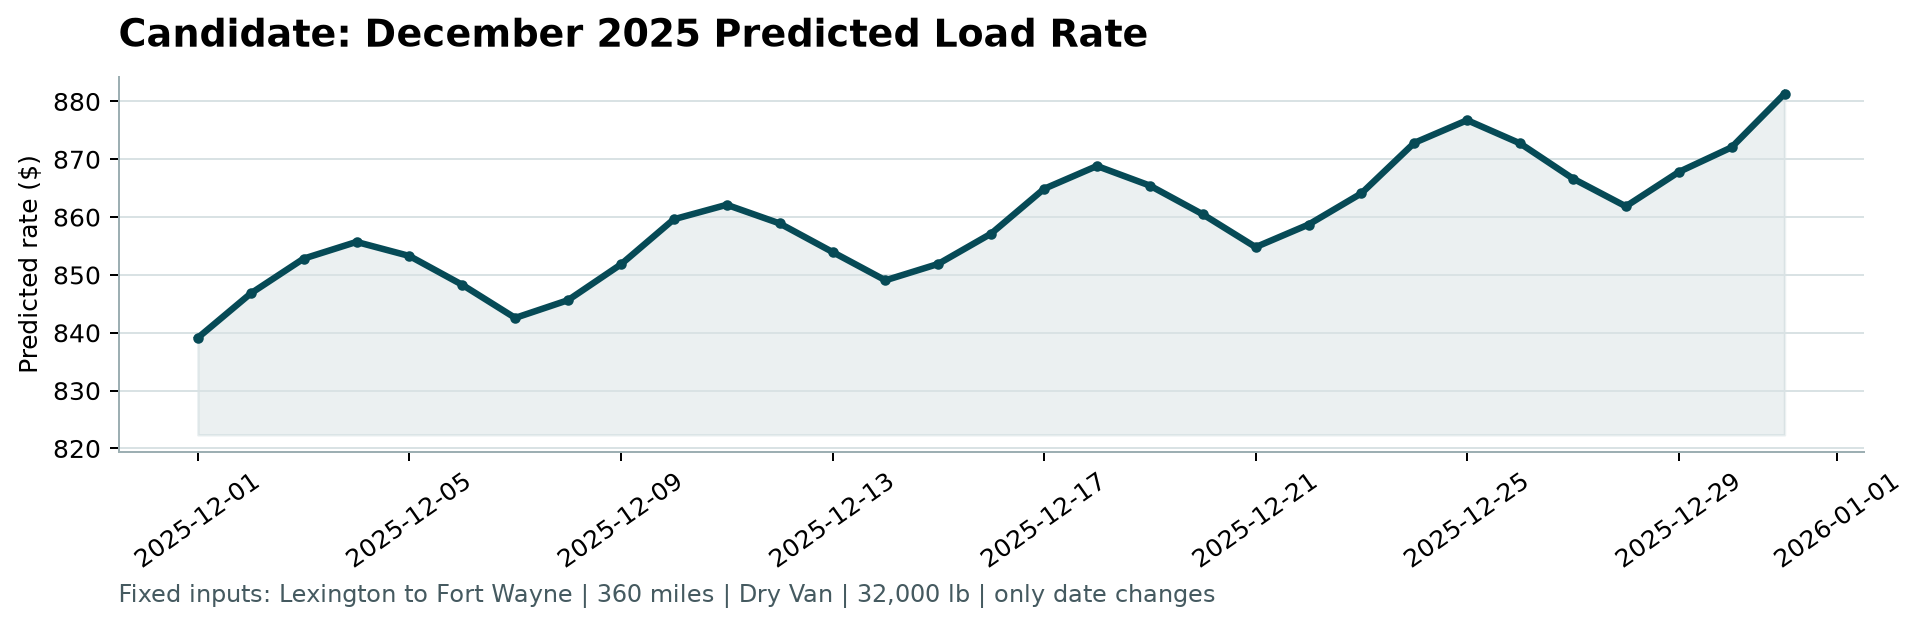
\includegraphics[width=0.92\linewidth]{candidate_december.png}
  \caption{December 2025 chart produced by \texttt{score.py} from the submitted predictions.}
\end{figure}

\section{Data and key findings}

\paragraph{Distance and equipment} Distance explains most of the price: the correlation is
\CorrClean{} once the corrupted labels are removed (\CorrRaw{} with them). Median rate per
mile is \RpmDV{} for Dry Van, \RpmFB{} for Flatbed and \RpmRF{} for Reefer. Price grows
less than proportionally with distance (log-log slope \DistSlope).

\paragraph{A daily market signal} \MI{} varies far more between days than within a day.
Its weekly cycle bottoms on Sunday and Monday and peaks on Thursday. It averages \MiTrain{} in
training and \MiVal{} in validation, so it is a genuine input for November--December. Its
price elasticity is \MiElast.

\paragraph{Time structure that \MI{} does not explain} Once \MI{} is controlled for, prices
still drift up about \Drift{} from January to October. They also climb through every
quarter-end month (March, June, September) and reset on the 1st. From the first day of the
month to the last, Flatbed rises \RampFB, Reefer \RampRF{} and Dry Van \RampDV{} (Figure~\ref{fig:time};
these are fitted values from the final model). December is a quarter-end month.

\begin{figure}[!htb]
  \centering
  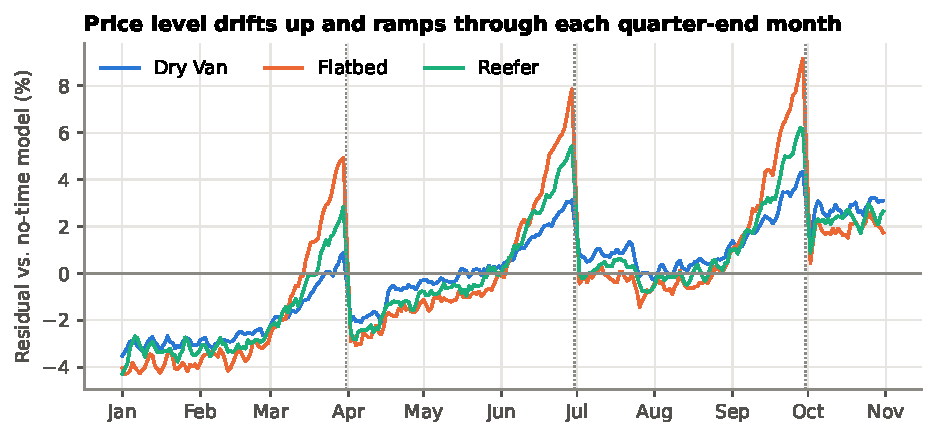
\includegraphics[width=0.94\linewidth]{time_structure.pdf}
  \caption{Daily mean residual by equipment from a model with no time terms (3-day mean).
    Dotted lines mark quarter ends.}
  \label{fig:time}
\end{figure}

\begin{figure}[!htb]
  \centering
  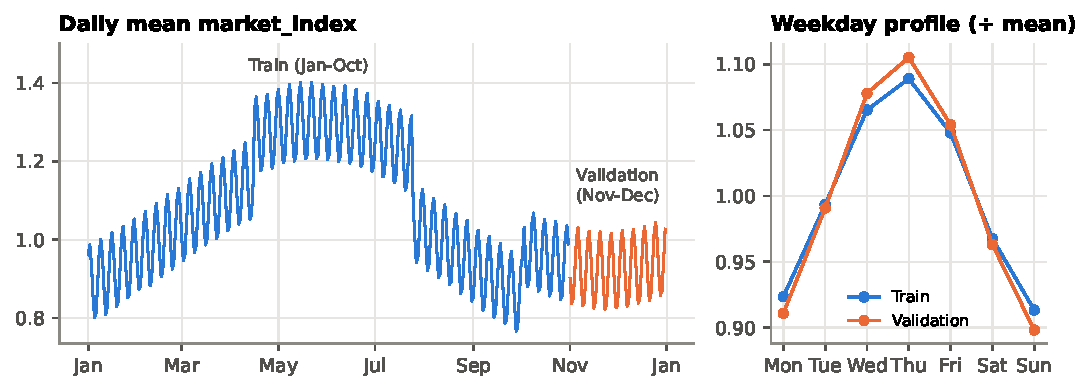
\includegraphics[width=\linewidth]{market_index.pdf}
  \caption{\MI{}: lower in November--December, with the same weekly cycle.}
\end{figure}

\paragraph{Unseen cities} Eight validation cities never appear in training (\NUnseen{}
rows, 12\%). In training, city effects are small (\CityLo{} to \CityHi), almost identical
whether the city is the pickup or the delivery ($r$ = \RPd), and they track latitude
($r$ = \RLat, Figure~\ref{fig:city}). A smooth function of the coordinates therefore
carries over to unseen cities. The coordinates are shifted from the real cities but are
consistent for each city, so they are used as given.

\begin{figure}[!htb]
  \centering
  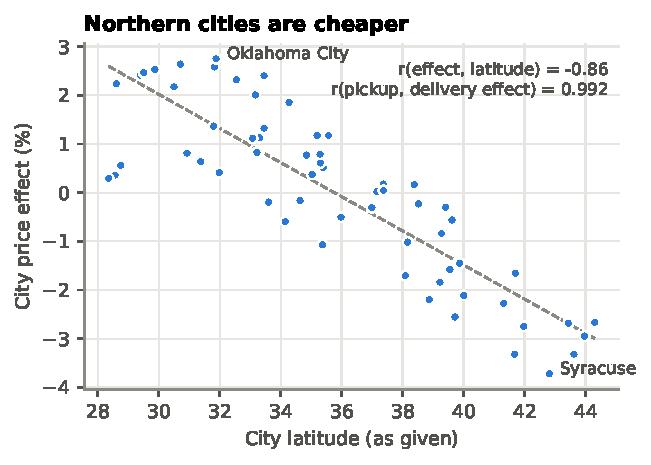
\includegraphics[width=0.5\linewidth]{city_effects.pdf}
  \caption{City price effect against latitude.}
  \label{fig:city}
\end{figure}

\paragraph{\QS{} is noise} Within lane $\times$ equipment groups, after weight, \MI{} and
time terms, adding \QS{} leaves the residual SD unchanged (\QsWithout{} without it,
\QsWith{} with it). Its apparent signal comes from the equipment mix. Adding it to the hybrid
worsens the fold-average MAE (\HybQsAvgMAE{} vs \HybAvgMAE), and removing it improves Codex's
LightGBM (\LgbmAvgMAE{} $\rightarrow$ \LgbmNoQsAvgMAE). It is dropped.

\section{Data-quality issues and fixes}

\begin{table}[!htb]
  \centering\small
  \begin{tabular}{@{}>{\raggedright\arraybackslash}p{0.44\linewidth}rr>{\raggedright\arraybackslash}p{0.33\linewidth}@{}}
\toprule
\textbf{Issue} & \textbf{Train} & \textbf{Validation} & \textbf{Handling} \\
\midrule
Weight missing & 300 & 165 & Fill with training median |weight|; w\_miss flag \\
Weight negative (sign flip) & 292 & 145 & Absolute value; w\_neg flag \\
Weight at cap $|w|$ = 47,500 & 1,204 & 301 & Keep (censored); w\_cap flag \\
\quad of which -47,500 & 13 & 4 & Absolute value \\
Weight at floor $|w|$ = 5,000 & 32 & 7 & Keep; w\_floor flag \\
market\_index missing & 374 & 249 & Fill with that date's mean \\
Distance at 70 mi floor & 48 & 21 & Keep (clipped, not an error) \\
Corrupted label (|log resid| $\geq$ 0.25) & 677 & --- & Dropped from training only (detector refitted inside each fold) \\
\quad high cluster (median $\times$3.33, range $\times$2.21-5.26) & 340 & --- &  \\
\quad low cluster (median $\times$0.29, range $\times$0.17-0.45) & 337 & --- &  \\
\bottomrule
\end{tabular}

  \caption{Data-quality rules: counts on the training and validation files, and how each is handled.}
\end{table}

Corrupted labels are found with a two-pass robust fit. The first pass fits the structural
model on log price with least squares. The second refits it on rows with
$|\text{residual}| < 0.30$. Rows with $|\text{residual}| \geq 0.25$ are then flagged. The
clusters are far from the clean rows: no residual falls between \GapLo{} and \GapHi{}
(Figure~\ref{fig:corrupt}), so cut-offs of 0.20, 0.25 and 0.30 flag the same rows.

The detector is refitted inside every fold, and flagged rows are removed from training
only; every validation row is predicted. The other repairs touch inputs only: missing values
get flags, so the model can learn whatever their absence means.

\begin{figure}[!htb]
  \centering
  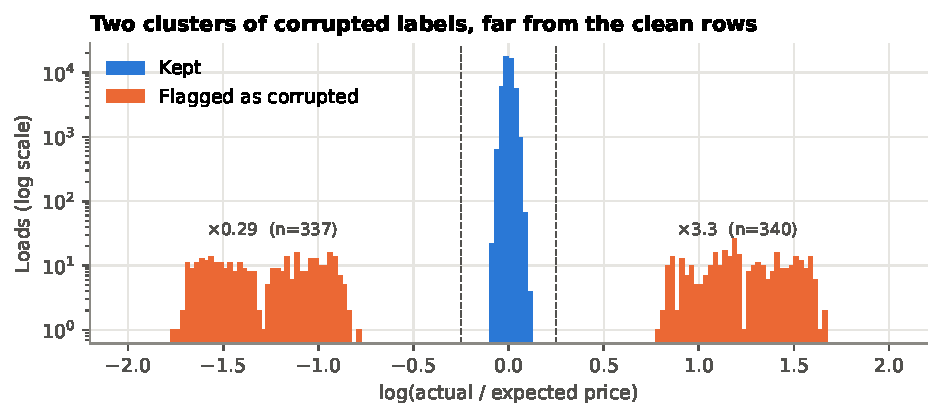
\includegraphics[width=0.94\linewidth]{corrupted_labels.pdf}
  \caption{$\log(\text{actual}/\text{expected})$ on the full training set (log count scale).}
  \label{fig:corrupt}
\end{figure}

\section{Split and validation approach}

The validation set is the two months after the training data, so every split looks forward
in time. Three expanding folds test August, September and October, each trained on all
earlier data. A fourth block, \textbf{h2}, trains through August and tests
September--October: like November--December, it is one to two months past the end of
training, and it spans a quarter end. Everything is refitted from scratch in each fold,
including the label cleaning and the weight imputation.

\begin{figure}[!htb]
  \centering
  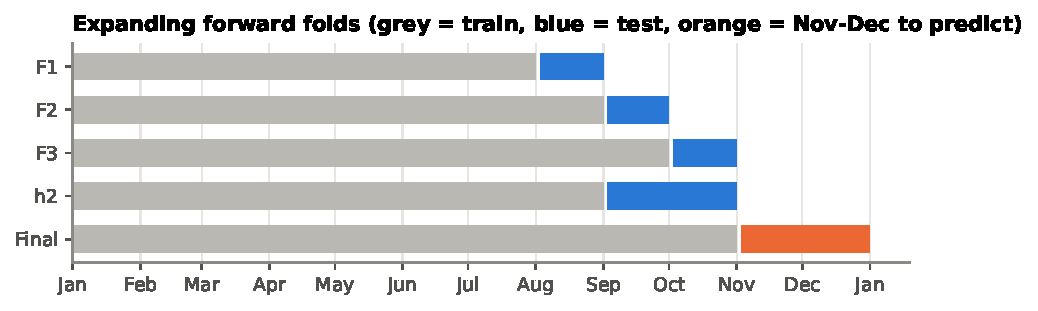
\includegraphics[width=0.9\linewidth]{folds.pdf}
  \caption{Folds. The final model trains on all of January--October.}
\end{figure}

Model selection used raw MAE averaged over F1--F3, with h2 MAE as the tie-break. Raw labels
include the corruption, as Spotter's labels presumably do, and MAE is robust to it. RMSE is
not: every model lands between \RmseMin{} and \RmseMax{}, because the corrupted rows
dominate the squared error. Clean-label MAPE (corrupted rows removed, for reporting only)
shows the accuracy on legitimate prices.

\begin{table}[!htb]
  \centering\small
  \begin{tabular}{@{}lrr@{}}
\toprule
\textbf{Split (MAE)} & \textbf{Hybrid} & \textbf{LightGBM-L1} \\
\midrule
Random 10\% holdout (all months) & \$91.5 & \$95.3 \\
Forward: train Jan--Sep, test Oct & \$95.4 & \$110.6 \\
Unseen cities: 8 withheld, test Sep--Oct & \$88.2 & \$110.6 \\
\bottomrule
\end{tabular}

  \caption{The same two models under three splits.}
\end{table}

A random split makes the two models look about equal (\RndHyb{} vs \RndLgbm). Going forward
in time, the tree model loses ground (\FwdHyb{} vs \FwdLgbm), so a random split would have
picked the wrong model. The unseen-city simulation withholds 8 training cities from
training and tests on the September--October loads that touch them. The hybrid holds up
(\UcHyb); the tree model, which relies on city identities, does not (\UcLgbm).

\section{Model}

\paragraph{Stage 1} Ordinary least squares on $\log(\PR)$, fitted on the cleaned rows. The
inputs are:
\begin{itemize}
  \item log distance;
  \item log weight, with a hinge term for loads under 12,000~lb, and a missing-weight flag;
  \item log \MI{} and equipment dummies;
  \item a quadratic surface in pickup and delivery coordinates;
  \item a linear trend in months;
  \item a quarter-end ramp per equipment: 0 on the first day of March, June, September or
    December, rising to 1 on its last day, and 0 in other months.
\end{itemize}

\paragraph{Stage 2} LightGBM on the stage-1 residuals. Its inputs are distance, weight,
\MI, equipment, coordinates, weekday, position within the month, and pickup and delivery
city as categorical features. It has no trend input, so it cannot undo the trend. Rows that
touch a city absent from training use a second stage-2 model without the city features.
The prediction is $\exp(\text{stage 1} + \text{stage 2})$.

\paragraph{Why not boosted trees alone} A tree predicts a constant beyond the last date it
saw, so it cannot carry the drift or a quarter-end ramp into the future. In the h2
backtest its error moves downward through the September ramp (Figure~\ref{fig:bias}), and
it cannot know that December will ramp. The linear stage carries time forward; the trees
handle the non-linear parts that do not depend on the date.

\begin{figure}[!htb]
  \centering
  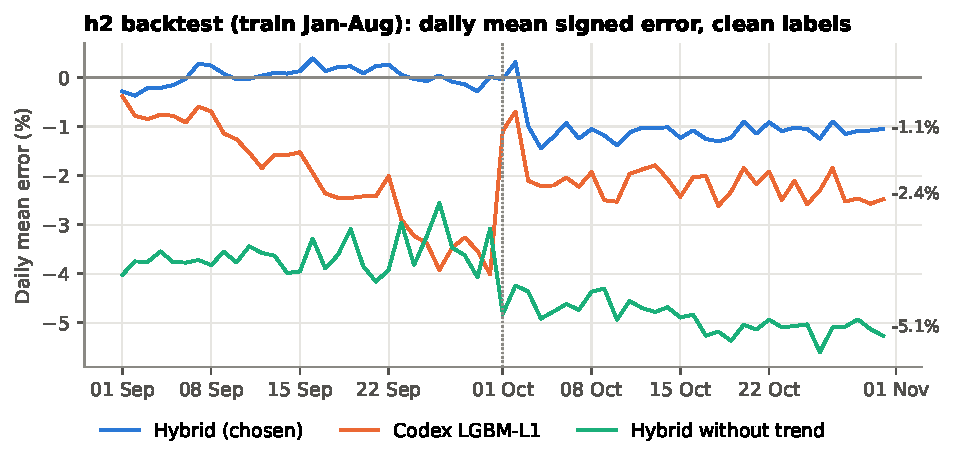
\includegraphics[width=0.9\linewidth]{backtest_bias.pdf}
  \caption{h2 backtest: daily mean signed error on clean labels (end labels show the
    last-5-day mean).}
  \label{fig:bias}
\end{figure}

\begin{table}[!htb]
  \centering\small
  \begin{tabular}{@{}lrrrrrrr@{}}
\toprule
\textbf{Model} & \textbf{Aug} & \textbf{Sep} & \textbf{Oct} & \textbf{h2} & \textbf{Fold avg} & \textbf{MAPE} & \textbf{Clean MAPE} \\
\midrule
\rowcolor{chosen}
\textbf{Hybrid (chosen)} & \textbf{79.9} & \textbf{80.4} & \textbf{95.4} & \textbf{88.5} & \textbf{85.2} & \textbf{3.83} & \textbf{1.33} \\
Hybrid, no city categoricals & 81.4 & 81.9 & 96.6 & 89.9 & 86.6 & 3.89 & 1.39 \\
Hybrid + quote\_signal & 85.4 & 79.9 & 94.9 & 87.9 & 86.7 & 3.90 & 1.40 \\
Hybrid, untuned defaults & 81.9 & 82.4 & 97.1 & 90.3 & 87.1 & 3.91 & 1.42 \\
Hybrid 50/50 with Codex XGB & 94.2 & 92.2 & 97.3 & 100.4 & 94.6 & 4.27 & 1.78 \\
Hybrid without quarter-end ramp & 94.4 & 107.3 & 90.5 & 102.5 & 97.4 & 4.33 & 1.83 \\
Structural only (stage 1) & 92.8 & 95.1 & 106.2 & 101.3 & 98.0 & 4.42 & 1.93 \\
Codex LGBM-L1 without quote\_signal & 85.3 & 116.2 & 107.2 & 117.6 & 102.9 & 4.64 & 2.16 \\
Codex blend 0.75 XGB / 0.25 LGBM & 118.2 & 115.6 & 107.2 & 118.9 & 113.7 & 5.09 & 2.63 \\
Codex LGBM-L1 & 119.5 & 111.4 & 110.6 & 114.8 & 113.8 & 5.08 & 2.62 \\
Codex XGB-L1 & 121.7 & 119.5 & 109.4 & 122.3 & 116.9 & 5.26 & 2.80 \\
Linear, city indicators, no time terms & 110.1 & 174.9 & 133.0 & 165.7 & 139.3 & 5.95 & 3.56 \\
Hybrid without trend & 120.8 & 136.1 & 163.7 & 154.2 & 140.2 & 6.05 & 3.68 \\
Hybrid without trend or ramp & 109.0 & 174.6 & 160.8 & 173.2 & 148.1 & 6.38 & 4.01 \\
Hybrid without market\_index & 197.3 & 205.8 & 101.1 & 169.2 & 168.1 & 7.41 & 4.85 \\
\bottomrule
\end{tabular}

  \caption{Forward-fold results. MAE in dollars on raw labels; MAPE and clean MAPE in
    percent, averaged over F1--F3. The Codex rows reproduce an earlier candidate solution:
    tree models on raw dollars with every feature, including \QS{} and calendar features.}
  \label{tab:models}
\end{table}

Removing the trend or \MI{} roughly doubles the error (Table~\ref{tab:models}), so handling time is the main problem.

\paragraph{Tuning} Before any tuning run, a small grid was committed to the repository,
along with the selection rule. The search went one setting at a time. It chose a linear
trend (over a step per quarter or a damped trend), 1,000 trees with 31 leaves, L2 loss, and
city categoricals. That improved the fold-average MAE from \HybUntunedAvgMAE{} to
\HybAvgMAE.

One change was made after tuning. The folds contain no unseen cities, and in the
unseen-city simulation the city categoricals made results worse (\UcNotRouted{} vs \UcHyb{}
with routing). So rows that touch an unseen city use the model without them; this leaves
every fold score unchanged. Results are stable across seeds (h2 MAE \SeedsHtwo).

\section{December prediction}

The chart inputs contain no \MI. Each December day gets the mean \MI{} of that day's loads
in \texttt{validation.csv}. This is an input feature Spotter supplied for the same dates,
not a label, and it is how the model is applied to the validation loads too. Dropping it
(with weekday dummies in its place) raises the h2 clean MAPE from \HybHtwoCMAPE{} to
\HybNoMiHtwoCMAPE.

The resulting chart reflects four things: the lower December \MI, the weekly cycle, the
continuing drift, and the Dry Van quarter-end ramp. It averages \DecMean. A Codex-style
LightGBM trained without \MI{} draws an almost flat line (\DecNoMiMin--\DecNoMiMax,
Figure~\ref{fig:dec}), because a tree has no way to extend time effects beyond October.

\begin{figure}[!htb]
  \centering
  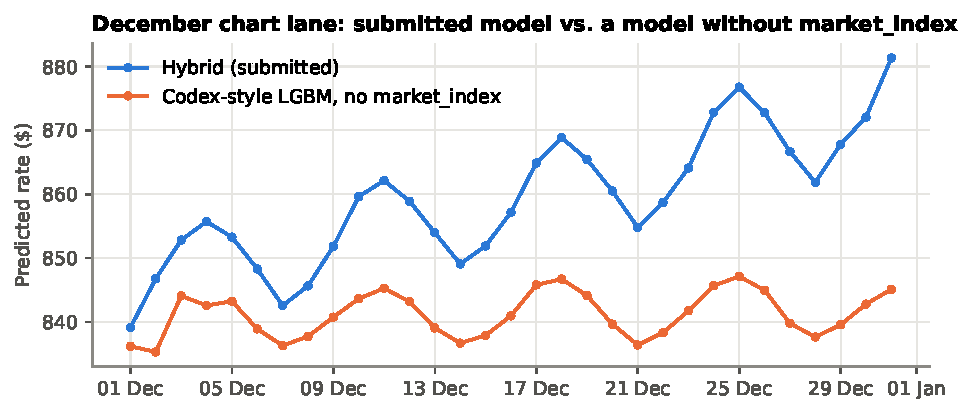
\includegraphics[width=0.86\linewidth]{december_crosscheck.pdf}
  \caption{December chart lane: the submitted hybrid against a tree model without \MI.}
  \label{fig:dec}
\end{figure}

\paragraph{Sanity checks} On the 12,000 validation predictions:
\begin{itemize}
  \item no value is missing or non-positive;
  \item median rate per mile is \PredRpmDV{} for Dry Van (training \RpmDV), \PredRpmFB{} for
    Flatbed (\RpmFB) and \PredRpmRF{} for Reefer (\RpmRF);
  \item rows touching an unseen city average \UnseenRpm/mi, against \SeenRpm/mi for the rest.
\end{itemize}

\section{Limitations and next steps}

\begin{itemize}
  \item \textbf{Extrapolation.} The linear trend and the December ramp are projected two
    months beyond the data. The ramp held in 3 of 3 quarters but cannot be checked for
    December. In the backtests the model under-predicted October, the month after a
    quarter end, by \HybOctBias.
  \item \textbf{Holidays.} Holiday effects in late December cannot be learned from
    January--October data.
  \item \textbf{Label corruption.} If the validation labels contain the same
    $\sim$\PctCorrupt{} corruption, raw MAE and especially RMSE will carry an error floor
    that no model can remove.
  \item \textbf{Next steps.} Quantile models for prediction intervals; drift monitoring on
    \MI{} and the residual level; monthly refits as new labels arrive; checking the
    corruption mechanism with the data owner.
\end{itemize}

\section*{Appendix: how to reproduce}

{\small
\begin{verbatim}
python -m pip install -r requirements.txt
python -m src.run_all            # full pipeline, about 6 minutes on 16 cores
python -m src.tune               # optional: rerun the pre-registered tuning grid
python score.py --predictions validation_predictions.csv \
                --december-predictions data/december_chart_inputs.csv
\end{verbatim}
}

{\small\raggedright
Code map: \texttt{src/clean.py} (input repairs, corrupted-label detector),
\texttt{src/models.py} (\texttt{HybridModel}, baselines), \texttt{src/validate.py} (folds,
metrics, contrasts), \texttt{src/tune.py} (pre-registered grid), \texttt{src/train.py} and
\texttt{src/predict.py} (final fit, outputs), \texttt{src/report.py} (this report; its numbers
are generated into \texttt{reports/generated/}). The README maps every file.

{\color{ink2}\Versions.}
}

\end{document}
